\documentclass{article}\usepackage[]{graphicx}\usepackage[]{color}
% maxwidth is the original width if it is less than linewidth
% otherwise use linewidth (to make sure the graphics do not exceed the margin)
\makeatletter
\def\maxwidth{ %
  \ifdim\Gin@nat@width>\linewidth
    \linewidth
  \else
    \Gin@nat@width
  \fi
}
\makeatother

\definecolor{fgcolor}{rgb}{0.345, 0.345, 0.345}
\newcommand{\hlnum}[1]{\textcolor[rgb]{0.686,0.059,0.569}{#1}}%
\newcommand{\hlstr}[1]{\textcolor[rgb]{0.192,0.494,0.8}{#1}}%
\newcommand{\hlcom}[1]{\textcolor[rgb]{0.678,0.584,0.686}{\textit{#1}}}%
\newcommand{\hlopt}[1]{\textcolor[rgb]{0,0,0}{#1}}%
\newcommand{\hlstd}[1]{\textcolor[rgb]{0.345,0.345,0.345}{#1}}%
\newcommand{\hlkwa}[1]{\textcolor[rgb]{0.161,0.373,0.58}{\textbf{#1}}}%
\newcommand{\hlkwb}[1]{\textcolor[rgb]{0.69,0.353,0.396}{#1}}%
\newcommand{\hlkwc}[1]{\textcolor[rgb]{0.333,0.667,0.333}{#1}}%
\newcommand{\hlkwd}[1]{\textcolor[rgb]{0.737,0.353,0.396}{\textbf{#1}}}%
\let\hlipl\hlkwb

\usepackage{framed}
\makeatletter
\newenvironment{kframe}{%
 \def\at@end@of@kframe{}%
 \ifinner\ifhmode%
  \def\at@end@of@kframe{\end{minipage}}%
  \begin{minipage}{\columnwidth}%
 \fi\fi%
 \def\FrameCommand##1{\hskip\@totalleftmargin \hskip-\fboxsep
 \colorbox{shadecolor}{##1}\hskip-\fboxsep
     % There is no \\@totalrightmargin, so:
     \hskip-\linewidth \hskip-\@totalleftmargin \hskip\columnwidth}%
 \MakeFramed {\advance\hsize-\width
   \@totalleftmargin\z@ \linewidth\hsize
   \@setminipage}}%
 {\par\unskip\endMakeFramed%
 \at@end@of@kframe}
\makeatother

\definecolor{shadecolor}{rgb}{.97, .97, .97}
\definecolor{messagecolor}{rgb}{0, 0, 0}
\definecolor{warningcolor}{rgb}{1, 0, 1}
\definecolor{errorcolor}{rgb}{1, 0, 0}
\newenvironment{knitrout}{}{} % an empty environment to be redefined in TeX

\usepackage{alltt}
\IfFileExists{upquote.sty}{\usepackage{upquote}}{}
\begin{document}

\begin{knitrout}
\definecolor{shadecolor}{rgb}{0.969, 0.969, 0.969}\color{fgcolor}\begin{kframe}
\begin{alltt}
\hlkwd{library}\hlstd{(readr)}
\hlstd{diabetes} \hlkwb{<-} \hlkwd{read_csv}\hlstd{(}\hlstr{"~/diabetes.csv"}\hlstd{)}
\end{alltt}


{\ttfamily\noindent\itshape\color{messagecolor}{\#\# \\\#\# -- Column specification --------------------------------------------------------\\\#\# cols(\\\#\# \ \ Pregnancies = col\_double(),\\\#\# \ \ Glucose = col\_double(),\\\#\# \ \ BloodPressure = col\_double(),\\\#\# \ \ SkinThickness = col\_double(),\\\#\# \ \ Insulin = col\_double(),\\\#\# \ \ BMI = col\_double(),\\\#\# \ \ DiabetesPedigreeFunction = col\_double(),\\\#\# \ \ Age = col\_double(),\\\#\# \ \ Outcome = col\_double()\\\#\# )}}\begin{alltt}
\hlkwd{head}\hlstd{(diabetes)}
\end{alltt}
\begin{verbatim}
## # A tibble: 6 x 9
##   Pregnancies Glucose BloodPressure SkinThickness Insulin   BMI DiabetesPedigre~
##         <dbl>   <dbl>         <dbl>         <dbl>   <dbl> <dbl>            <dbl>
## 1           6     148            72            35       0  33.6            0.627
## 2           1      85            66            29       0  26.6            0.351
## 3           8     183            64             0       0  23.3            0.672
## 4           1      89            66            23      94  28.1            0.167
## 5           0     137            40            35     168  43.1            2.29 
## 6           5     116            74             0       0  25.6            0.201
## # ... with 2 more variables: Age <dbl>, Outcome <dbl>
\end{verbatim}
\begin{alltt}
\hlkwd{attach}\hlstd{(diabetes)}
\end{alltt}
\end{kframe}
\end{knitrout}
\begin{knitrout}
\definecolor{shadecolor}{rgb}{0.969, 0.969, 0.969}\color{fgcolor}\begin{kframe}
\begin{alltt}
\hlkwd{View}\hlstd{(diabetes)}
\hlkwd{na.omit}\hlstd{(diabetes)}
\end{alltt}
\begin{verbatim}
## # A tibble: 768 x 9
##    Pregnancies Glucose BloodPressure SkinThickness Insulin   BMI
##          <dbl>   <dbl>         <dbl>         <dbl>   <dbl> <dbl>
##  1           6     148            72            35       0  33.6
##  2           1      85            66            29       0  26.6
##  3           8     183            64             0       0  23.3
##  4           1      89            66            23      94  28.1
##  5           0     137            40            35     168  43.1
##  6           5     116            74             0       0  25.6
##  7           3      78            50            32      88  31  
##  8          10     115             0             0       0  35.3
##  9           2     197            70            45     543  30.5
## 10           8     125            96             0       0   0  
## # ... with 758 more rows, and 3 more variables: DiabetesPedigreeFunction <dbl>,
## #   Age <dbl>, Outcome <dbl>
\end{verbatim}
\end{kframe}
\end{knitrout}

\begin{knitrout}
\definecolor{shadecolor}{rgb}{0.969, 0.969, 0.969}\color{fgcolor}\begin{kframe}
\begin{alltt}
\hlstd{diabetes}\hlkwb{<-}\hlkwd{scale}\hlstd{(diabetes)}
\hlkwd{head}\hlstd{(diabetes,}\hlnum{10}\hlstd{)}
\end{alltt}
\begin{verbatim}
##       Pregnancies    Glucose BloodPressure SkinThickness    Insulin        BMI
##  [1,]   0.6395305  0.8477713    0.14954330     0.9066791 -0.6924393  0.2038799
##  [2,]  -0.8443348 -1.1226647   -0.16044119     0.5305558 -0.6924393 -0.6839762
##  [3,]   1.2330766  1.9424580   -0.26376935    -1.2873733 -0.6924393 -1.1025370
##  [4,]  -0.8443348 -0.9975577   -0.16044119     0.1544326  0.1232213 -0.4937213
##  [5,]  -1.1411079  0.5037269   -1.50370731     0.9066791  0.7653372  1.4088275
##  [6,]   0.3427574 -0.1530851    0.25287146    -1.2873733 -0.6924393 -0.8108128
##  [7,]  -0.2507887 -1.3416021   -0.98706650     0.7186174  0.0711579 -0.1258952
##  [8,]   1.8266227 -0.1843619   -3.57027057    -1.2873733 -0.6924393  0.4195021
##  [9,]  -0.5475618  2.3803327    0.04621514     1.5335512  4.0193026 -0.1893135
## [10,]   1.2330766  0.1284058    1.38948126    -1.2873733 -0.6924393 -4.0578295
##       DiabetesPedigreeFunction         Age    Outcome
##  [1,]                0.4681869  1.42506672  1.3650064
##  [2,]               -0.3648230 -0.19054773 -0.7316434
##  [3,]                0.6040037 -0.10551539  1.3650064
##  [4,]               -0.9201630 -1.04087112 -0.7316434
##  [5,]                5.4813370 -0.02048305  1.3650064
##  [6,]               -0.8175458 -0.27558007 -0.7316434
##  [7,]               -0.6756927 -0.61570943  1.3650064
##  [8,]               -1.0197620 -0.36061241 -0.7316434
##  [9,]               -0.9473263  1.68016374  1.3650064
## [10,]               -0.7239831  1.76519608  1.3650064
\end{verbatim}
\end{kframe}
\end{knitrout}

\begin{knitrout}
\definecolor{shadecolor}{rgb}{0.969, 0.969, 0.969}\color{fgcolor}\begin{kframe}
\begin{alltt}
\hlkwd{library}\hlstd{(cluster)}
\hlkwd{library}\hlstd{(factoextra)}
\end{alltt}


{\ttfamily\noindent\itshape\color{messagecolor}{\#\# Loading required package: ggplot2}}

{\ttfamily\noindent\itshape\color{messagecolor}{\#\# Welcome! Want to learn more? See two factoextra-related books at https://goo.gl/ve3WBa}}\end{kframe}
\end{knitrout}

\begin{knitrout}
\definecolor{shadecolor}{rgb}{0.969, 0.969, 0.969}\color{fgcolor}\begin{kframe}
\begin{alltt}
\hlkwd{fviz_nbclust}\hlstd{(diabetes,kmeans,}\hlkwc{method}\hlstd{=}\hlstr{"wcss"}\hlstd{)}
\end{alltt}


{\ttfamily\noindent\bfseries\color{errorcolor}{\#\# Error in match.arg(method): 'arg' should be one of "{}silhouette"{}, "{}wss"{}, "{}gap\_stat"{}}}\begin{alltt}
\hlkwd{fviz_nbclust}\hlstd{(diabetes,kmeans,}\hlkwc{method}\hlstd{=}\hlstr{"gap_stat"}\hlstd{)}
\end{alltt}


{\ttfamily\noindent\color{warningcolor}{\#\# Warning: did not converge in 10 iterations}}\end{kframe}
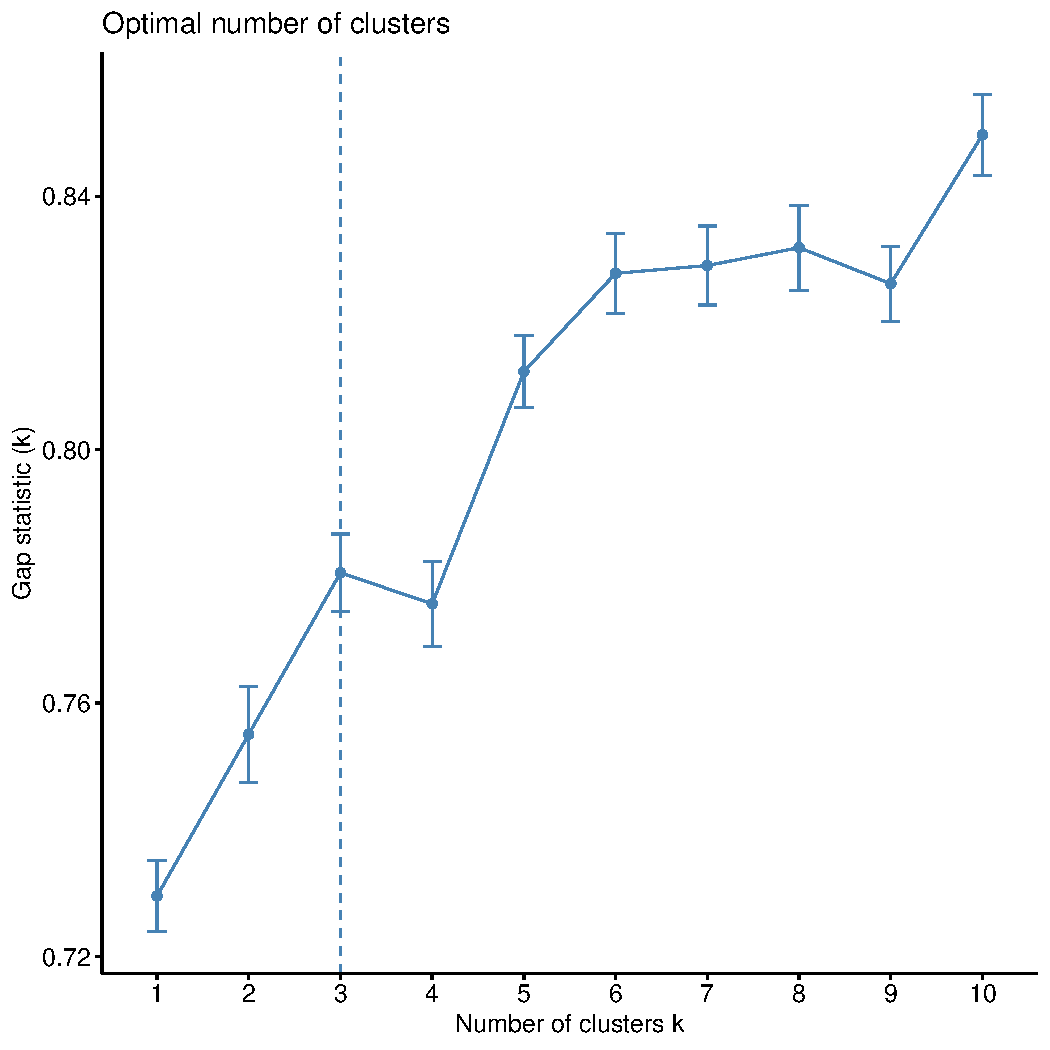
\includegraphics[width=\maxwidth]{figure/unnamed-chunk-5-1} 
\end{knitrout}

\end{document}
